%% Dokumentklasse KOMA-Script Report
\documentclass[paper=a4, 12pt]{scrreprt}
%% Encoding UTF8
\usepackage[utf8]{inputenc}
%% 8 Bit Aufloesung der Buchstaben
\usepackage[T1]{fontenc}
%% Seitenraender
\usepackage[scale=0.72]{geometry}
%% Spracheinstellungen
\usepackage[english, naustrian]{babel} % your native language must be the last one!!
%% erweiterte Farbenpalette
\usepackage[dvipsnames]{xcolor}
%% Abbildungen
\usepackage{graphicx}
%% Tabellen (erweitert)
\usepackage{tabularx}
%% TikZ + Circuit-TikZ (fuer Schaltungen)
\usepackage[europeanresistors, europeaninductors]{circuitikz}
%% Nuetzliche TikZ Libraries
\usetikzlibrary{arrows, automata, positioning}
%% mathematik
\usepackage{amsmath, amssymb}
%\usepackage{mathtools}	
%% pdf-einbindung
\usepackage{pdfpages}
%% scource-code einbindung
\usepackage{listings, scrhack} %scrhack vermeidet Umschaltung auf KOMA Floats..
\usepackage{courier}
%% euro-symbol
\usepackage{eurosym}
%% landcsape-seiten ermöglichen
\usepackage{lscape}

%% Diplomarbeits-Format
\usepackage{srdpdipa}

%% Abkuerzungsverzeichnis
\usepackage[]{acronym}

%% Todos
\usepackage[]{todonotes}

%% Ganttdiagramme
\usepackage{pgfgantt}



% Hyperlinks im Dokument
\usepackage[colorlinks=true,
    linkcolor=black,
    citecolor=green,
    bookmarks=true,
    urlcolor=black,
    bookmarksopen=true]{hyperref}

\begin{document}
Hier kommt das Labor-Deckblatt hin
%\includepdf[pages=-]{.pdf}


%% inhaltsverzeichnis ==================================%%
\tableofcontents
%%======================================================%%

\newpage

%%Grundsätzliche Erklärungen===============================================%%
\chapter{Aufgabenstellung}
Das Ziel von dem Projekt war es, eine intelligente Lüftersteuerung mit Web-Application zu entwerfen.
Ein Temperatursensor liefert die Temperaturen an ein ESP-Modul, welches die Daten per WLAN weiter sendet an einen RaspberryPi. Der RaspberryPi dient als Server und verwaltet die Daten. Mit Hilfe einer Web-Application werden die gemessenen Werte in einem Diagramm ausgegeben. Werden Temperaturen über einer gewissen Schwelle gemessen, schaltet sich der Lüfter ein. Hat sich die Temperatur normalisiert wird der Lüfter wieder abgeschaltet.

\section{Realisierung}
Das ESP-Modul dient als Client und der RaspberryPi als Broker.
Damit das ESP-Modul Daten senden kann muss es eine stabile Verbindung zu einem vorhandenen WLAN-Netzwerk haben. Falls die Verbindung zum WLAN oder zum Broker abbricht schalten sich zwei Warn-LEDs ein. Eine dritte LED geht an, falls es zu heiß wird und der Lüfter eingeschaltet werden muss. 
Zur sicheren Übertragung der Werte, wird das MQTT-Protokoll (Message Queuing Telemetry Transport) verwendet. Der Pi bekommt die Daten und wertet diese mit Hilfe von Python aus.\textbf{ RAPHIS PART}

\textbf{BILD CLIENT WLAN BROKER DATENBANK}

%%Infos ESP=====================================================%%
\chapter{ESP-Modul}
\section{Übersicht}
Modul mit WLAN verbinden, Daten senden und empfangen mit Arduino IDE kompatibel, Warum ESP verwendet,
\section{Technische Daten}
Zur Realisierung wurde das Entwicklerboard \textit{NodeMCU Lua Lolin V3 Module ESP8266} verwendet. Es besitzt ein WLAN-Funkmodul mit einer integrierten 25dBm Antenne.
Programmiert wird es über eine Micro-USB Schnittstelle und ist mit der Arduino IDE kompatibel. Die Versorgung des Moduls funktioniert über die Schnittstelle sowie mit einem externen Netzgerät oder einer Batterie. Obwohl das Entwicklerboard im Normalfall 3V3 kompatibel ist, kann es auch mit 5V versorgt werden da es einen internen Spannungswandler besitzt. \textbf{https://www.bastelgarage.ch/esp8266-nodemcu-v3-kompatibles-development-board}

%%Pining ESP Modul=====================================%%
\begin{center}
\begin{minipage}{0.5\textwidth}
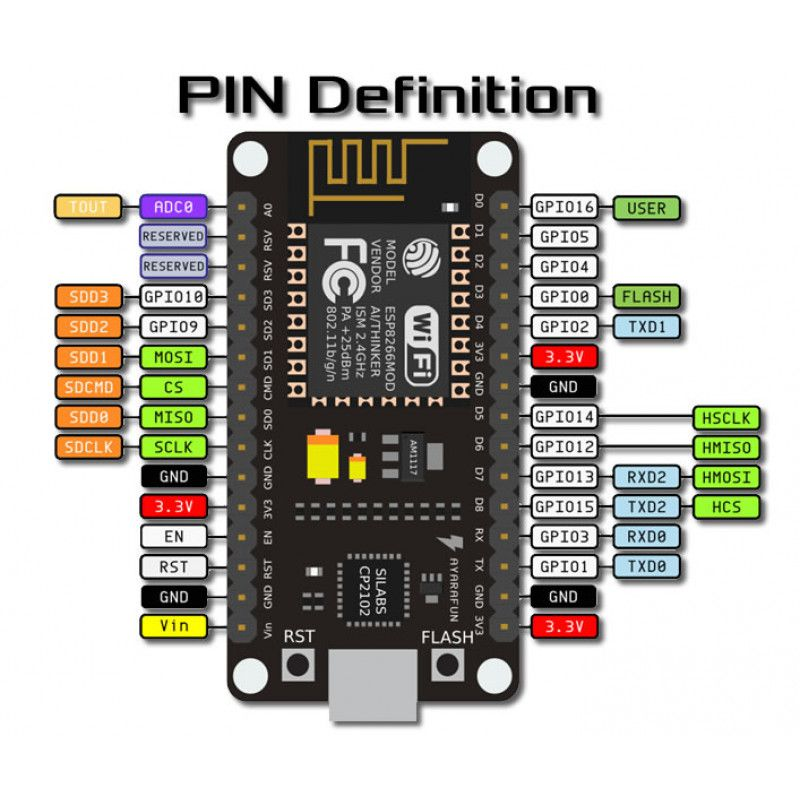
\includegraphics[width=0.7\textwidth]{ESP_pining.jpg} 
\end{minipage}\hfill% 
\begin{minipage}{0.5\textwidth}
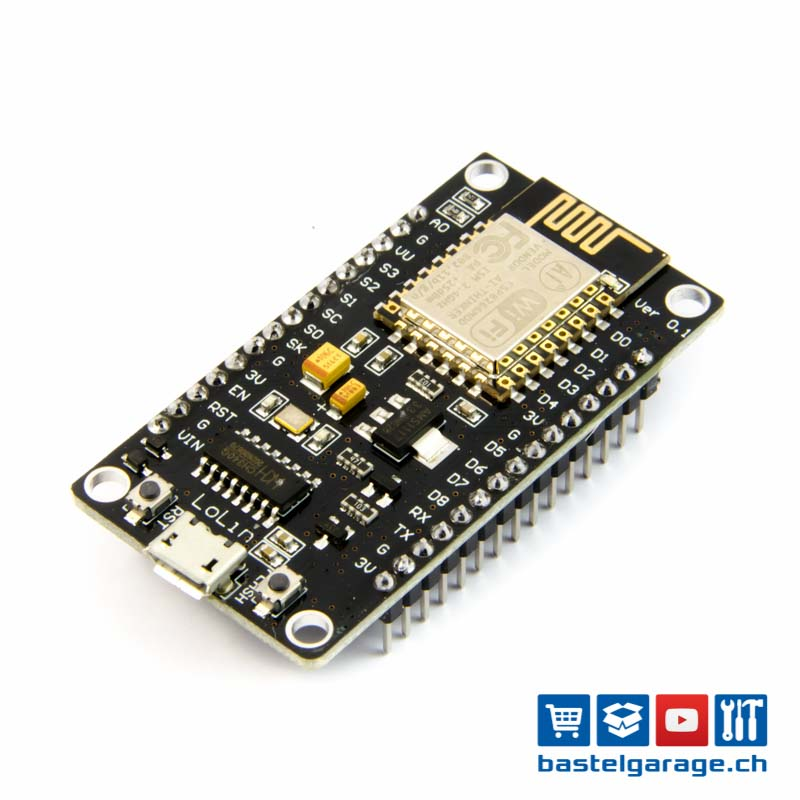
\includegraphics[width=0.7\textwidth]{Entwicklerboard.jpg} 
\end{minipage}
\end{center}

\section{(Verbindung mit) Temperatursensor}
serieller Monitor

\chapter{Konfigurationen}
\section{ESP8266 als Client}
\section{Virtual Machine als Broker}
\subsection{MQTT}
Publishen und Subcriben
\section{Verbindungsaufbau}
Einfaches senden und empfangen auf terminal

\chapter{Erweiterungen} 
\section{Warn-LEDs}
Einfaches Blockschal bild/ selbst gezeichnetes auf zettel, noch nicht in altium
\section{Lüfter}
\section{Display}
\section{Sleep Mode}
\section{Aufbau auf Lochrasterplatte}
Altium Schaltung

\chapter{Raspberry Pi}
\textbf{RAPHIS PART}
\section{Übersicht}
\section{Technische Daten}
\chapter{Pi als Broker}
\section{MQTT}
\section{Daten empfangen}
\chapter{WebOberfläche}
\section{Daten in Diagramm ausgeben}

\chapter{ESP2 Daten empfangen}
\section{Ausgabe auf Display}
Temp-Sensor drausen sendet Daten zu Pi, der sendet Daten weiter zu zweitem ESP-Modul mit Display wo man Temperatur ablesen kann(Wenn Pi in anderem Raum wie bennötigtes Display)

\end{document}
